\documentclass{article}

\usepackage{tikz}
\usetikzlibrary{calc,3d,arrows,shapes}
\usepackage{tikz-3dplot}
\usepackage{amsmath}
\usepackage{amsfonts}
\usetikzlibrary{external}
\tikzexternalize % activate!
\begin{document}



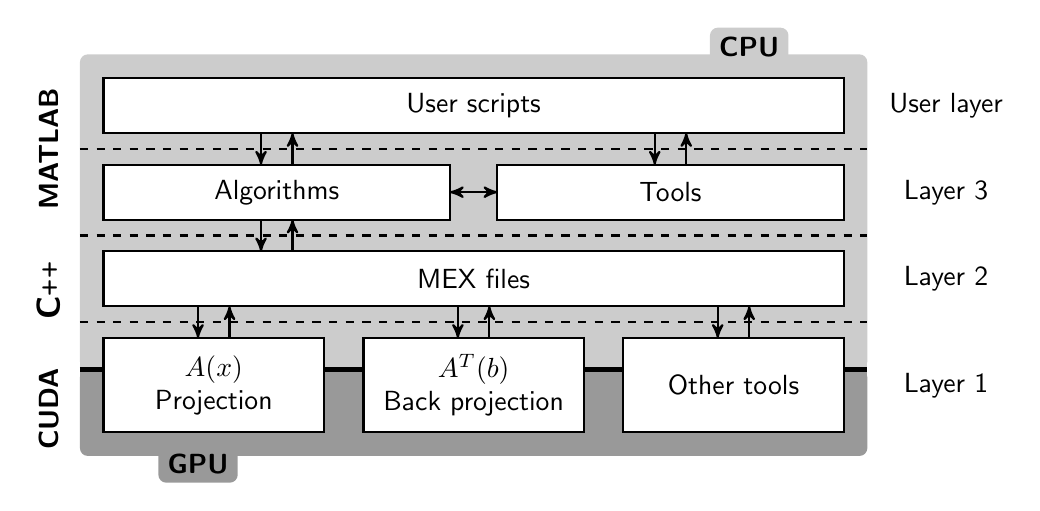
\begin{tikzpicture}[>=stealth',           % arrow tip
                    xscale=1,              % scale
                    font=\sffamily
                    ]  
                    
\fill[rounded corners=1mm,black!20] (0,-0.2) rectangle (10,3.8); 
\fill[,black!20] (0,-0.2) rectangle (10,3); 

\fill[rounded corners=1mm,black!40] (0,-1.3) rectangle (10,-0.2); 
\fill[black!40] (0,-1) rectangle (10,-0.2); 

\node[rounded corners=1mm,fill=black!40] at (1.5,-1.4) {\textbf{GPU}};
\node[rounded corners=1mm,, fill=black!20] at (8.5,3.9) {\textbf{CPU}};
\draw[ultra thick](0,-0.2) -- (10,-0.2);

\node[rotate=90] at (-0.4,2.6) {\textbf{MATLAB}};
\node[rotate=90] at (-0.4,0.8) {\large \textbf{C\texttt{++}}};
\node[rotate=90] at (-0.4,-0.7) {\textbf{CUDA}};

% User Scripts
\draw[thick,black,fill=white] (0.3,3.5) rectangle (9.7,2.8); 
 \node at (5,3.15) {User scripts};
\draw[dashed, thick](0,2.6) -- (10,2.6);
 \node at (11,3.15) {User layer};


% Algorithms 
 \draw[thick,->](2.3,2.8) -- (2.3,2.4);
 \draw[thick,<-](2.7,2.8) -- (2.7,2.4);
 
 \draw[thick,black,fill=white] (0.3,2.4) rectangle (4.7,1.7); 
 \node at (2.5,2.05) {Algorithms};        
  \node at (11,2.05) {Layer 3};


 % tools 
 \draw[thick,->](7.3,2.8) -- (7.3,2.4);
 \draw[thick,<-](7.7,2.8) -- (7.7,2.4);
 \draw[thick,<->](4.7,2.05) -- (5.3,2.05);
 \draw[thick,black,fill=white] (5.3,2.4) rectangle (9.7,1.7); 
 \node at (7.5,2.05) {Tools};  
            
% Mex FILES            
  \draw[thick,black,fill=white] (0.3,1.3) rectangle (9.7,0.6); 
 \node at (5,0.95) {MEX files};
\draw[dashed, thick](0,1.5) -- (10,1.5);          
 \draw[thick,->](2.3,1.7) -- (2.3,1.3);
 \draw[thick,<-](2.7,1.7) -- (2.7,1.3);
   \node at (11,0.95) {Layer 2};

 
\draw[dashed, thick](0,0.4) -- (10,0.4);
 
 
 
 %2.8 withd each
 \node at (11,-0.4) {Layer 1};
 % Projection 
\draw[thick,black,fill=white] (0.3,0.2) rectangle (3.1,-1); 
 \node[align=center] at (1.7,-0.4) {$A(x)$ \\ Projection};
\draw[thick,<-](1.5,0.2) -- (1.5,0.6);
 \draw[thick,->](1.9,0.2) -- (1.9,0.6);



 % Back projection
 \draw[thick,black,fill=white] (3.6,0.2) rectangle (6.4,-1); 
 \node[align=center] at (5,-0.4) {$A^T(b)$ \\ Back projection};
\draw[thick,<-](4.8,0.2) -- (4.8,0.6);
 \draw[thick,->](5.2,0.2) -- (5.2,0.6);
 
 %others
 \draw[thick,black,fill=white] (6.9,0.2) rectangle (9.7,-1); 
 \node[align=center] at (8.3,-0.4) {Other tools};
\draw[thick,<-](8.1,0.2) -- (8.1,0.6);
 \draw[thick,->](8.5,0.2) -- (8.5,0.6);
 
 
\end{tikzpicture}
\end{document}
